\documentclass[cs4size,a4paper,nofonts]{ctexart}
\usepackage[utf8]{inputenc}
\def\tjf{田劲锋}
\def\titlec{从“三起三落”谈对邓小平的评价 }
\usepackage[top=25.4mm,bottom=25.4mm,left=31.8mm,right=31.8mm]{geometry} % 页面设置
\usepackage[unicode,breaklinks=true,
colorlinks=true,linkcolor=black,anchorcolor=black,citecolor=black,urlcolor=black,
pdftitle={\titlec},pdfauthor={\tjf}]{hyperref}
\usepackage{xeCJK}
\usepackage{xpinyin}

\usepackage{multicol} % 分栏
\usepackage{multirow} % 跨行
\usepackage{longtable} % 长表格
\usepackage{graphicx} % 图形
\usepackage{color} % 颜色
\usepackage{xcolor} % 颜色
\usepackage{url} % 排版链接
\usepackage{nameref}
\usepackage{caption}
\captionsetup{font={small}} % 标题字体大小
\usepackage[inline]{enumitem} % 调整列表样式

\setmainfont{Times New Roman}
\setCJKmainfont[BoldFont={SimHei}]{SimSun}  % 主要字体:宋体、黑体
\setCJKsansfont[BoldFont={STZhongsong}]{STFangsong} % 次要字体:仿宋、中宋
\setCJKmonofont{KFKai} % 等宽字体:楷体
\setCJKfamilyfont{msyh}[BoldFont={* Bold}]{微软雅黑} \newcommand{\msyh}{\CJKfamily{msyh}} % 微软雅黑
\setCJKfamilyfont{mincho}{MS PMincho} \newcommand{\mincho}{\CJKfamily{mincho}} % 文泉驿微米黑
\setCJKfamilyfont{fangso}{华文仿宋} \newcommand{\fangso}{\CJKfamily{fangso}} % STLiti
\setCJKfamilyfont{xingkai}{华文行楷} \newcommand{\xingkai}{\CJKfamily{xingkai}}

\CJKsetecglue{\hspace{0.1em}}
\renewcommand\CJKglue{\hskip -0.3pt plus 0.08\baselineskip}
\frenchspacing
\widowpenalty=10000
\linespread{1.5} % 1.5 倍行距
\setlength{\parskip}{2pt plus 2pt}
\renewcommand{\baselinestretch}{1.5}

\setlength{\abovecaptionskip}{1pt}
\setlength{\belowcaptionskip}{0pt}
\setlength{\intextsep}{8pt}
\setlist{topsep=0pt,partopsep=0pt,itemsep=0pt,parsep=0pt}

\makeindex
\pagestyle{plain}

\begin{document}

%%%% 开始 %%%%

\begin{titlepage}

% 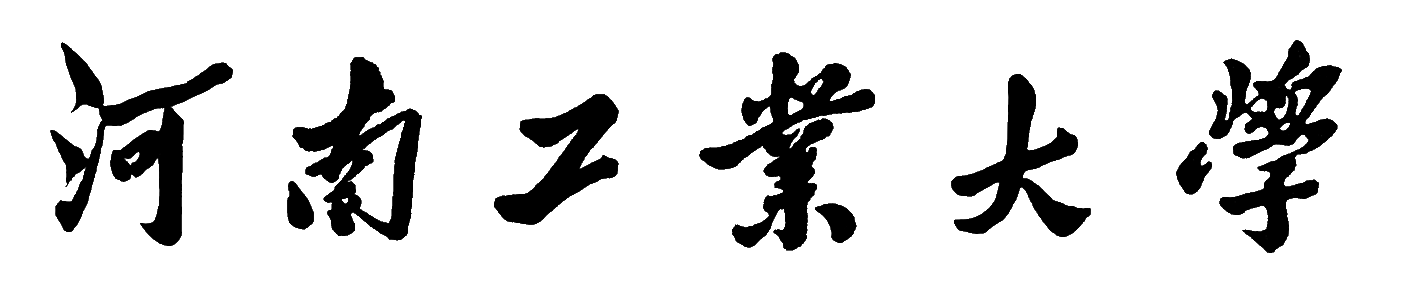
\includegraphics[height=20.4mm]{images/haut.png}

\begin{center}

{\sf\bfseries\zihao{-2}{毛泽东思想与中国特色社会主义理论体系概论

实践调研论文}}

\vspace*{1cm}


\includegraphics[height=21.4mm]{images/hautlogo.png}

\vspace*{1cm}

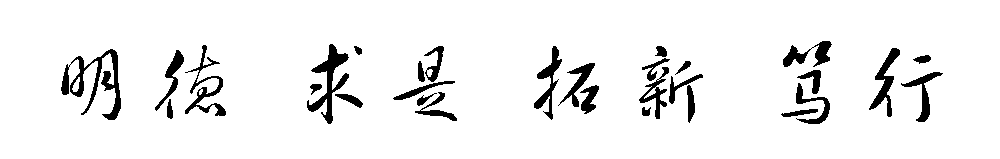
\includegraphics[height=25.1mm]{images/xiaoxun.png}

\vspace*{1cm}

{\sf\bfseries\zihao{-2} 得分:\underline{\makebox[5em][c]{}}}

\vfill
{\large
\newcommand{\ctline}[2]{\makebox[4em][s]{\bf #1}:\underline{\makebox[15em][c]{#2}}\par}
\newcommand{\ctlin}[2]{\makebox[4em][s]{\bf #1}\quad\underline{\makebox[15em][c]{#2}}\par}
\ctline{论文名称}{\titlec}
\ctline{年级专业}{软件 1305 班}
\ctline{小组名称}{第 6 组}
\ctline{评阅教师}{赵排风}
\ctline{提交时间}{2014--2015学年第2学期}
}

\end{center}

\end{titlepage}

\begin{abstract}
成功对于每个人都不是偶然的。作为中国第二代领导人的邓小平,正是历经人生“三起三落”的洗礼,磨砺自己的意志,坚定自己革命信念,走上人生的顶峰,成为全军全党全国各族人民公认的享有崇高威望的卓越领导人,伟大的马克思主义者,伟大的无产阶级革命家,中国社会主义改革开放和现代化建设的总设计师,而他的成功也因他“三起三落”而变得更加耀眼灿烂。

{\bf 关键字:} 邓小平;中国;领导人;社会主义。
\end{abstract}

邓小平1904年出生在四川广安,1920年,赴法国勤工留学,较早地接触到马克思主义思想,不久加入共产主义组织,走上了革命道路。1929年,受中央委派,赴广西领导百色起义、龙州起义,开辟左右江革命根据地。1933年,邓小平迎来了人生的“一落”,邓小平拥护毛泽东提出的“以农村包围城市、武装夺取政权”革命道路的坚定实践者,为此受到了当时“左”倾路线的迫害。他和毛泽覃、谢唯俊、古柏等人拥护毛泽东为代表的正确路线,坚决主张建立农村革命根据地,反对“城市中心论”,反对“左”的土地分配政策,结果被当时党内的“左”倾领导者撤职,被打成所谓的“邓、毛、谢、古反党集团”,为此,邓小平遭批斗,职务也被撤销,并受到党内最严重警告处分。然而这并没有消磨邓小平的革命意志,邓小平依然坚持自己心中的革命信念,终于,遵义会议后,确定了毛泽东领导地位,邓小平也恢复了一切职务。一起一落,邓小平的这一切经历更为后来的革命道路奠定了坚强的基础。
  
1966年,文化大革命期间,邓小平作为“刘邓资产阶级司令部”的第二号“走资派”被打倒,被剥夺一切职务,全家受到株连,1969年10月,邓小平被下放到江西新建县,在当地拖拉机修造厂劳动。在江西的三年,他读了许多马列著作和古今中外的书籍,并结合中国实际,对什么是社会主义、怎样建设社会主义的问题作了更深入的思考。1971年9月,林彪反革命政变阴谋被粉碎。1973年,毛泽东重新起用邓小平,并恢复其国务院副总理职务。毛泽东称赞他“政治思想强”,“人才难得”,“柔中有刚,绵里藏针”。邓小平受命于危难之时,再次从严重的政治挫折中崛起。1975年1月,邓小平担任中央副主席、国务院副总理、中央军委副主席、中国人民解放军总参谋长,主持党、国家和军队的日常工作。

在此期间由于邓小平召集军队干部会、省市委书记会、农业会议、科学院会议,系统地提出了全面整顿的思想。这些会议的中心议题都是“整顿”。全面整顿,就是全面纠正“文化大革命”的错误,把党的工作重点转移到四个现代化建设上来。整顿实际上是后来改革的实验。整顿的实质是系统纠正“文化大革命”的错误,矛头直指“四人帮”。由此,邓小平再次受到错误路线的打击,被指责为搞“右倾翻案风”,再次被错误地撤消党内外一切职务。这是他政治生涯中的第三次严重挫折。1976年9月9日,毛泽东在北京逝世,举国哀悼。同年10月6日,“四人帮”被粉碎,长达十年的“文化大革命”结束,举国欢腾。悲喜之际,全国人民都关注着毛泽东之后中国的前途和命运。在1977年3月的中央工作会议上,陈云、王震提出要邓小平出来工作。7月,党的十届三中全会恢复了邓小平在1976年被错误撤消的一切领导职务。邓小平第三次从严重的政治挫折中崛起。

正是在大起大落的经历后,邓小平才更彻底的看清一切,1978年十一届三中全会开辟了中国改革开放和集中力量进行社会主义现代化建设的新时期。

20世纪80年代初,邓小平在论述怎样才能发挥社会主义制度优越性的问题时,第一次提出了社会主义本质这个概念,邓小平指出:“社会主义是一个很好的名词,但是如果搞不好,不能正确理解,不能采取正确的政策,那就体现不出社会主义的本质。”那么,应该怎么“正确理解”社会主义呢?他认为,讲社会主义,首先要使生产力发展,只有这样,才能表明社会主义的优越性;社会主义经济政策对不对,归根到底要看生产力是否发展,人民收入是否增加。邓小平把“发展生产”和“增加人民收入”称之为压倒一切的标准,实际上已经提出了社会主义本质的核心内容。同时,邓小平还对不符合社会主义本质要求的思想进行了深刻的剖析提出“四个不是”和“一个没有”的观点,即:“贫穷不是社会主义,发展太慢不是社会主义,平均主义不是社会主义,两极分化也不是社会主义”,“一个没有”就是“没有民主就没有社会主义”。

1986年9月,提出“社会主义本质论断的雏形”,邓小平指出:“社会主义财富属于人民,社会主义的致富是全民共同致富。社会主义原则,第一是发展生产,第二是共同致富。”这段话成为社会主义本质论断的雏形。1990年12月,提出共同富裕是社会主义最大的优越性。

1990年12月,邓小平又一次强调共同富裕的问题。他指出:“共同致富,我们从改革一开始就讲,将来总有一天要成为中心课题。社会主义不是少数人富起来,大我数人穷,不是那个样子。社会主义最大的优越性就是共同富裕,这是体现社会主义本质的一个东西。”

1992年初,邓小平在南方谈话中明确提出关于社会主义本质的著名论断。

1979年3月,他在党的理论工作务虚会上的讲话中强调指出:“现在搞建设,也要适合中国情况,走出一条中国式的现代化道路。”

同年10月,他在谈到实现现代化时第一次明确提出要修改原来关于现代化的具体目标。他说:“我们开了大口,本世纪末实现四个现代化。后来改了个口,叫中国式的现代化,就是把标准放低一点。特别是国民生产总值,按人口平均来说不会很高。”

1979年12月,他第一次使用了“小康”的概念。“小康社会”是千百年来中国人民所熟悉的一个概念,邓小平同志指出:“所谓小康,从国民生产总值来说,就是年人均达到八百美元”,这样就必须是国民生产总值达到一万亿美元,“这一万亿美元,反映到人民生活上,我们就叫小康水平;反映到国力上,就是较强国家”。他指出:“所谓小康社会,就是虽不富裕,但日子好过。我们是社会主义国家,国民收入分配要使所有的人都得益,没有太富的人,也没有太穷的人,所以日子普遍好过。更重要的是,那时我们可以进入国民生产总值达到一万亿美元以上的国家的行列,这样的国家不多。”

1980年1月,他把到20世纪末的20年分为两个10年,初步提出分“两步走”达到“小康水平”的战略构想。这个战略构想,后来在五届全国人大四次会议和党的十二大的报告中得到肯定。

党的十二大正式提出分两步走,20世纪末在不断提高经济效益的前提下,工农业总产值翻两番,实现小康社会的经济发展战略,并确定了我国经济建设的战略目标、战略重点、战略步骤和一系列正确方针。

20世纪末,人民生活总体上达到小康水平以后,再往前发展的战略目标是什么?在党的十二大召开前夕,邓小平曾指出,如果能实现小康社会的目标,我们就取得了一个新的起点,再花30年到50年时间,接近发达国家的水平。我们不是说赶上,更不是说超过,而是接近。

1987年2月,邓小平更切合实际地把接近发达国家水平改为,到21世纪中叶我们建成中等发达水平的社会主义国家。

正是邓小平坚持改革开放,中国取得举世瞩目的成就,经济特区的划分,引进外资,使沿海一带快速地发展起来,我国第一个经济特区被称为为“一夜崛起之城”,经济特区的建立成功引进外资和先进技术,先进的管理经验,扩大了我们走向了世界的通道,如今经济特区的繁荣正是验证的这一切,因此中国经济得以快速发展。
一国两制的建立,实现了香港澳门的回归,相信在不久的将来,台湾也将回归祖国的怀抱。

科技发展,邓小平坚持科技发展观,大力发展科学技术,坚持创新新国家,为中国发展奠定了很好的基础。

邓小平,在经历三起三落后依然坚定自己心中火热信念,一心为中国的发展建设付出了自己的一生,带领中国走向了富强。你的三起三落更加增添了你身上的独特魅力,作为中国社会主义改革开放和现代化建设的总设计师,你得到了全中国人们的拥戴,你永远活在了我们心中。

%%%% 结束 %%%%

\end{document}
